\documentclass{amsart}
\usepackage{amsthm}
\usepackage{enumerate}
\usepackage{xcolor}
\usepackage{tikz}
   \usetikzlibrary{calc} 
\usepackage{float}
\usepackage{wrapfig}

\theoremstyle{definition}
\newtheorem{theorem}{Theorem}
\newtheorem{problem}{Problem}
\newtheorem{corollary}{Corollary}
\newtheorem{remark}{Remark}
\newtheorem{conjecture}{Conjecture}
\newtheorem{lemma}{Lemma}
\newtheorem{step}{Step}
\newtheorem{case}{Case}
\newtheorem{definition}{Definition}
\newtheorem{proposition}{Proposition}
\newcommand{\ncc}{c}

\begin{document}
\author{Gao Mou}
\address{School of Physical and Mathematical Sciences, Nanyang Technological University, Singapore} 
\email{gaom0002@e.ntu.edu.sg} 
\author{Dmitrii V. Pasechnik}
\address{Department of Computer Science, The University of Oxford, UK}
\email{dimpase@cs.ox.ac.uk}

\title{Edge-dominating cycles, $k$-walks and Hamilton prisms in $2K_2$-free graphs}
\begin{abstract}
We show that every $\frac{1}{k-1}$-tough
$2K_2$-free graph admits a $k$-walk, and it can be found in polynomial time.
For this class of graphs, this proves a
long-standing conjecture due to Jackson and Wormald (1990).
Furthermore, we prove that every $(1+\epsilon)$-tough $2K_2$-free graph is prism-Hamiltonian,
along with few other similar results.
\end{abstract}

\maketitle

\section{Introduction}
A graph $G$ is called $\beta$-{\em tough}, for a real $\beta>0$, if for any $p\geq 2$ it
cannot be split into $p$ components by removing less than $p\beta$ vertices.  
This concept, a measure of graph connectivity and ``resilience'' under vertex subsets removal,
was introduced in 1973 by V. Chv\'{a}tal 
while studying   Hamiltonicity of graphs. For a survey of results on graph toughness till 2006
cf. \cite{MR2221006}.

Let $p\times G$ denote the multigraph obtained from $G$ by taking each edge $p$ times. 
A $k$-{\em walk} is a spanning subgraph $W$ of $2k\times G$, such that each vertex of $W$ 
has even degree at most $2k$. % (the evenness says that $W$ is Eulerian). 
In particular a graph has a $1$-walk if and only if it is $K_2$ (i.e. one edge) or Hamiltonian.
In 1990 B.~Jackson and N.~Wormald conjectured \cite{jackson1990k} that for any integer $k\ge2$ a
$\frac{1}{k-1}$-tough graph $G$ admits a $k$-walk.
{For a survey of results on walks in graphs till 2005 cf. \cite{kouider2005connected}.}

In this paper, we prove that Jackson and Wormald's Conjecture is true, under the
assumption that $G$ is  $2K_2$-free, that is $G$ does not contain an induced
copy of the disjoint union of two edges. 

\begin{theorem}\label{thm2} 
For any integer $k\ge2$, every $\frac{1}{k-1}$-tough $2K_2$-free graph $G$
admits a $k$-walk.
Moreover, the latter can be found in time polynomial in $|V(G)|$.
\end{theorem}

If for $k\geq 2$ we let the toughness value $\frac{1}{k-1}$ increase to
$\frac{1}{k-2}$ then
one does not need $2K_2$-freeness. Indeed, it is shown in
\cite{jackson1990k} that
every $\frac{1}{k-2}$-tough graph has a $k$-walk.

Clearly, if $G$ is
Hamiltonian, then $G$ is 1-tough.  More generally,
If $G$ has a $k$-walk, then $G$ is $\frac{1}{k}$-tough \cite{jackson1990k}.
However, the converse is not true already for $k=1$ (there even exist $2$-tough graphs which are
not Hamiltonian, cf. \cite{bauer2000not}).

This more or less summarises the situation with $t$-tough graphs, $t\leq 1$.
On the $t>1$ side 
a famous conjecture of V.~Chv\'{a}tal \cite{chvatal1973tough} claims
that there exists a constant $\beta$ such that every
$\beta$-tough graph is Hamiltonian.  
Towards this, 
M.~Ellingham and X.~Zha \cite{ellingham2000toughness} proved that
every 4-tough graph has a 2-walk (cf. Theorem~\ref{thm1} below).

Recently, in \cite{broersma2014toughness}, H.~Broersma, V.~Patel and A.~Pyatkin proved that 
every 25-tough 2$K_2$-free graph on at least three vertices is Hamiltonian.
Our Theorem~\ref{thm2} was inspired by this result.  
However, our approach is technically quite different. 

\newpage

The {\em prism} over a graph $G$ is the Cartesian product 
\begin{wrapfigure}[6]{r}{.3\textwidth}
\centering
\setlength{\unitlength}{.5mm}
\begin{picture}(50,40)%(60,50)
\put(10,10){\circle*{1.5}}
\put(20,10){\circle*{1.5}}
\put(40,10){\circle*{1.5}}
\put(50,10){\circle*{1.5}}
\put(30,20){\circle*{1.5}}
\put(30,30){\circle*{1.5}}
\put(10,10){\line(1,0){40}}
\put(20,10){\line(1,1){10}}
\put(30,20){\line(1,-1){10}}
\put(30,20){\line(0,1){10}}
\end{picture}
\label{fignoprism}
\end{wrapfigure}
$G\square K_2$ of $G$ with the complete graph $K_2$. 
$G$ is called 
{\em prism-Hamiltonian} if $G\square K_2$ is Hamiltonian. 
If $G$ is Hamiltonian, then $G\square K_2$ is also Hamiltonian, but the converse does not hold in general, 
cf. \cite{kaiser2007hamilton}. 
As well, this property is stronger than having a $2$-walk: cf. figure on the right, where
we have a 
$2K_2$-free graph with  a $2$-walk, but without Hamiltonian prism.

Our next result is as follows.
\begin{theorem}\label{thm1}
Every $(1+\epsilon)$-tough $2K_2$-free graph $G$ is prism-Hamiltonian, for any $\epsilon>0$.
\end{theorem}

To prove Theorem~\ref{thm2} and Theorem \ref{thm1}, we first prove
\begin{theorem}\label{addgen1} 
Let $G$ be a $2K_2$-free graph. Then
\begin{enumerate}
\item $G$ admits an edge-dominating cycle (or an edge, or a vertex) $C$; 
\item if $G$ contains a triangle, then $G$ admits 
an edge-dominating cycle $C$, with three successive vertices on $C$ forming a triangle in $G$. 
\end{enumerate}
Moreover, $C$ can be found in time polynomial in $|V(G)|$.
\end{theorem}

In fact, in 1983 Veldman \cite{veldman83} has proved the existence of
edge-dominating cycles for $2K_2$-free graphs. However, his proof is based on
contraposition, so neither tells how to find $C$ in (1), nor
allows to restrict $C$ as in (2).

The terminology we use is  mostly from \cite{bomu08}; we include the following for the sake of
clarity.  
A {\em clique} means a complete subgraph, a {\em coclique} means a
induced subgraph containing no edge. 
For any
$v\in V$, let $v^\perp:=v^{\perp_G}$ denote the union of $\{v\}$ and the set of
neighbours of $v$ in $G$.  More generally, for $A\subset V$, let
$A^\perp:=A^{\perp_G}$ denote the set of vertices {\em dominated} by $A$, i.e.
$A^\perp=\bigcup\limits_{y\in A}v^\perp$, and $A$ is said to be {\em
dominating} if $A^\perp=V$.
Moreover, if $A^{\perp}=V$ and the induced subgraph $V-A$ is a coclique, then we say $A$ is {\em edge-dominating}. 
 
It should also lead to no confusion when we talk
about  dominating induced subgraphs $H$ of $G$, in the sense of $V(H)$ being
dominating, respectively a subset of vertices (e.g. set of vertices of a
subgraph) being dominated by $H$, etc.


%\begin{proposition}\label{veldman2}{\cite[Theorem 2]{veldman83}}
%Let $G$ be a graph other than a tree, if for every pair of remote edges $e$ and $f$ of $G$.
%$$$d(e)+d(f)\ge|V(G)|-2,$$
%then $G$ admits an edge-dominating cycle.
%\end{proposition}







\section{Proof of Theorem \ref{addgen1}}

\subsection{The proof of the first part of Theorem \ref{addgen1}}
If $G$ is a tree, then, as it is $2K_2$-free, it must either have an edge-dominating
vertex, or an edge-dominating edge.
Otherwise, $G$ has a cycle, say $C=x_1x_2\cdots x_kx_1$, where $k\ge3$.
If $C$ is edge-dominating, then we are done. 
%%%% - to continue editing here:
Now assume $C$ is not edge-dominating. Then, there must be some edge $v_1v_2$ (assume there are $t$ such edges), with neither $v_1$ nor $v_2$ is on $C$. 
Since $G$ is $2K_2$-free, $v_1$ and $v_2$ have at least two neighbors on $C$. Otherwise, if there is at most one vertex on $C$ adjacent to $v_1$ or $v_2$, then a $2K_2$ will appear.

Now, assume $x_1v_1\in E(G)$, 
\begin{enumerate}
\item if $x_2v_1\in E(G)$, then $C'=x_1v_1x_2x_3\cdots x_kx_1$ is a longer cycle,
\item if $x_2v_2\in E(G)$, then $x_1v_1v_2x_2x_3\cdots x_kx_1$ is a longer cycle, 
\item if $x_2v_1,x_2v_2\not\in E(G)$, then apply the $2K_2$-free property to $v_1v_2$ and $x_2x_3$, we get either $x_3v_1\in E(G)$ or $x_3v_2\in E(G)$.
\begin{enumerate}
\item if $x_3v_2\in E(G)$, then $C'=x_1v_1v_2x_3\cdots x_kx_1$ is a longer cycle,
\item if $x_3v_2\not\in E(G)$, then $x_3v_1\in E(G)$.
\begin{enumerate}
\item if $x_2$ is adjacent to no vertex outside $C$, then we use $C'=x_1v_1x_3\cdots x_kx_1$ to instead $C$. We know that $C$ and $C'$ have the same length, but $C'$ dominates all the edges who are dominated by $C$, and $C'$ also dominates $v_1v_2$, who is not dominated by $C$. So $t$ becomes smaller.
\item if $x_2$ is adjacent to some vertices outside $C$, say $z$, for example.

Recall that $x_2$ is adjacent to neither $v_1$ nor $v_2$, then $z$ must be adjacent to either $v_1$ or $v_2$. If $zv_1\in E(G)$, then $C'=x_1v_1zx_2x_3\cdots x_kx_1$ is a longer cycle.
If $zv_2\in E(G)$, then $C'=x_1v_1v_2zx_2x_3\cdots x_kx_1$ is a longer cycle.
\end{enumerate}

\end{enumerate}
\end{enumerate}

Repeat the process above. We know the length of a cycle in $G$ is limited, then the process will stop in finite steps. Finally, there will be no edge independent with the cycle from the last step. That is the edge-dominating cycle we want.

\qed

\subsection{The proof of the second part of Theorem  \ref{addgen1}}
The proof of the second part is almost the same with the first, only needing a little modification.

Suppose a $2K_2$-free graph $G$ is not a tree, and contains a triangle, namely $w_1w_2w_3$.
If $w_1w_2w_3$ is edge-dominating, then there is nothing to prove. Otherwise, there is an edge, namely $u_1u_2\in E(G)$, with neither $u_1$ nor $u_2$  on $w_1w_2w_3$. Then, by the $2K_2$-freeness, we can connect $w_1w_2w_3$ and $u_1u_2$ together, to get a 5-cycle, with $w_1$, $w_2$ and $w_3$ successive (the order is possibly changed). 

If such a 5-cycle is edge-dominating, then we have finished the proof. Otherwise, we are going to prove the following statement. 

Suppose $G$ contains a cycle $C$ of length $|V(C)|=k$, for $k\ge5$, and there are three successive vertices on $C$, namely $X'$, $X$ and $X''$ forming a triangle in $G$. If $C$ is not edge-dominating, then we can find a cycle $C'$ such that either $C'$ is edge-dominating or $C'$ dominates more edges than $C$. What is more, $X'$, $X$ and $X''$ are also successive on $C'$.

Assume that $e=v_1v_2$ is an edge of $G$ such that neither $v_1$ nor $v_2$ is on $C$. By $2K_2$-freeness, $v_1$ and $v_2$ are adjacent to at least two of $\{X,X',X''\}$, then at least one of $\{X',X''\}$. Suppose $v_1X'\in E(G)$, then we label the vertices in $C$ in the following way.

$X'$ is labeled by $x_1$. The neighbor of $x_1$ (on $C$), who is not $X$, is labeled by $x_2$. Other vertices on $C$ is labeled successively. Then, certainly, $X''$ is labeled by $x_{k-1}$ and $X$ is labeled by $x_k$. See the following picture (Figure \ref{labelcycle}).

\begin{figure}[h]
\begin{center}
\caption{The cycle $C$ of length $k$}\label{labelcycle}
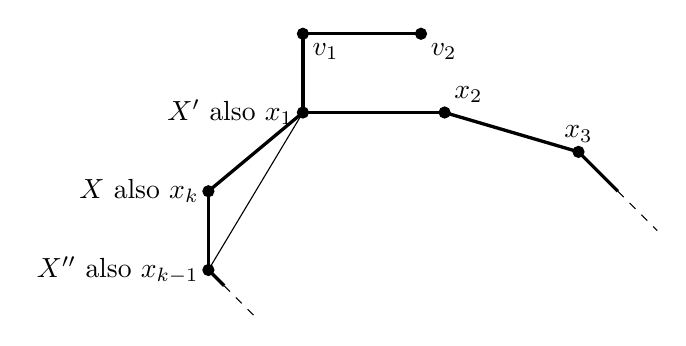
\begin{tikzpicture}


\filldraw[black](0,0)node[left]{$X'$ also $x_1$} circle(2pt);
\filldraw[black](1.8,0)node[above right]{ $x_2$} circle(2pt);
\filldraw[black](3.5,-0.5)node[above]{ $x_3$} circle(2pt);
\draw[very thick](0,0)--(1.8,0);
\draw[very thick](3.5,-0.5)--(1.8,0);
\draw[very thick](3.5,-0.5)--(4,-1);
\draw[dashed](4,-1)--(4.5,-1.5);

\filldraw[black](-1.2,-1)node[left]{$X$ also $x_k$} circle(2pt);
\draw[very thick](0,0)--(-1.2,-1);

\filldraw[black](-1.2,-2)node[left]{$X''$ also $x_{k-1}$} circle(2pt);
\draw[very thick](-1.2,-2)--(-1.2,-1);
\draw[very thick](-1.2,-2)--(-1,-2.2);
\draw[dashed](-1,-2.2)--(-0.6,-2.6);

\filldraw[black](0,1)node[below right]{ $v_1$} circle(2pt);
\draw[very thick](0,1)--(1.5,1);
\filldraw[black](1.5,1)node[below right]{ $v_2$} circle(2pt);
\draw[very thick](0,1)--(0,0);
\draw[thin](0,0)--(-1.2,-2);



\end{tikzpicture}
\end{center}
\end{figure}

Note that the operation (in the proof of the first part of Theorem \ref{addgen1}) of enlarging the cycle $C$ to $C'$ has nothing to do with the edges $x_{k-1}x_k$ and $x_kx_1$ when $k\ge5$. Thus the three vertices $X''$, $X$ and $X'$ are always successive on the cycle in our process. Then they are on the edge-dominating cycle we found finally.




















\qed


\section{Proof of Theorem \ref{thm2}}





The following lemma is the key technique in the proof of Theorem \ref{thm2}.

\begin{lemma}\label{addtec}
If $G$ has an edge-dominating cycle and if $G$ is $\frac{1}{k-1}$-tough, then $G$ admits a $k$-walk.
\end{lemma}

\begin{proof}
Denote the edge-dominating cycle as $C$, thus the induced subgraph $D=G-C$ is a coclique. For any subset $D_0\subset D$, by $\frac{1}{k-1}$-toughness, $D_0$ has at least $\lceil\frac{|D_0|}{k-1}\rceil$ neighbors in $C$. By Hall' Theorem, there is $E'\subset E(G)$ such that each $e\in E'$ has one vertex in $D$ and the other in $C$. And each vertex in $D$ is incident to exactly one edge in $E'$, while each vertex in $C$ is incident to at most $k-1$ edges in $E'$. Then these (doubled) edges in $E'$ and the edges in the edge-dominating cycle $C$ form a $k$-walk in $G$.
\end{proof}

Now, let us come back to the proof of Theorem \ref{thm2}.

If $G$ is a tree, and $G$ is $\frac{1}{k-1}$-tough, then obviously, for each $v\in V(G)$, the degree $d(v)\le k-1$. So, we can double each edge in $G$ to get the $k$-walk (in fact a $(k-1)$-walk).
If $G$ is not a tree, then
combining Lemmas \ref{addtec}  and Theorem \ref{addgen1},
we obtain Theorem \ref{thm2}.
\qed


\medskip

Now, let us state two conjectures to close this section.
\begin{conjecture}
Every $3/2$-tough $2K_2$-free graph with at least 3 vertices has a 2-trail, i.e. a 2-walk with each edge appearing in the walk at most once.
\end{conjecture}


\begin{conjecture}
Every 2-tough $2K_2$-free graph with at least 3 vertices is Hamiltonian.
\end{conjecture}









\section{The proof of Theorem \ref{thm1}}

The following lemma is the key technique in the proof of Theorem \ref{thm1}.
\begin{lemma}\label{keylem}
Suppose $G$ is $(1+\epsilon)$-tough, for some $\epsilon>0$.
\begin{enumerate}
\item If $G$ contains an edge-dominating cycle $C$ with even number of vertices, then the prism of $G$ is Hamiltonian.
\item If $G$ contains an edge-dominating cycle $C=v_1v_2\cdots v_{2p+1}v_1$ of odd length, and there are three vertices $v_1$, $v_{2q}$ and $v_{2q+1}$, for some $0\le q\le p$, inducing a triangle in $G$, then the prism over $G$ is Hamiltonian.
\end{enumerate}
\end{lemma}

\begin{proof}
For the first part (see the following picture), denote the (even size) edge-dominating path in $G$ by $C=v_1v_2\cdots v_{2p}v_1$. The set of vertices outside the path $D=V(G)-V(C)$ is an independent set. By Hall's Theorem and 1-toughness, there is a matching $M$, from $D$ to $C$. That means for any vertex $u_j$ in $D$, there is a vertex $v_{i_j}$ on $C$ adjacent to $u_j$ in $M$.

Obviously, we have a Hamilton cycle in $\bar{C}$, the prism over $C$, namely $$v_1v'_1v'_2v_2\cdots v_{2p-1}v'_{2p-1}v'_{2p}v_{2p}v_1.$$ Now, we change every  $v_{i_j}v'_{i_j}$ (or $v'_{i_j}v_{i_j}$) into $v_{i_j}u_ju'_jv'_{i_j}$ (or $v'_{i_j}u'_ju_jv_{i_j}$) to get a Hamilton cycle in $\bar{G}$.

\begin{figure}[h]
\caption{$G$ has an edge-dominating cycle of even length}
\begin{center}
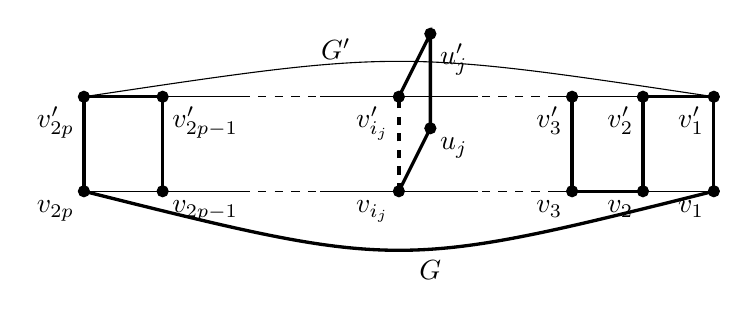
\begin{tikzpicture}[scale=2]
\draw(-2,0)node[below left]{$v_{2p}$}--(-1,0);\draw(-0.5,0)--(0.5,0);\draw(1,0)--(2,0);
\draw(-2,0.6)node[below left]{$v'_{2p}$}--(-1,0.6);\draw(-0.5,0.6)--(0.5,0.6);\draw(1,0.6)--(2,0.6);
\filldraw[black](0,0)node[below left]{$v_{i_j}$} circle(1pt);
\filldraw[black](0,0.6)node[below left]{$v'_{i_j}$} circle(1pt);
\filldraw[black](-2,0.6) circle(1pt);
\filldraw[black](2,0.6)node[below left]{$v'_1$} circle(1pt);
\filldraw[black](-1.5,0.6)node[below right]{$v'_{2p-1}$} circle(1pt);
\filldraw[black](1.55,0.6)node[below left]{$v'_2$} circle(1pt);
\filldraw[black](2,0)node[below left]{$v_1$} circle(1pt);
\filldraw[black](-2,0) circle(1pt);
\filldraw[black](1.55,0)node[below left]{$v_2$} circle(1pt);
\filldraw[black](-1.5,0)node[below right]{$v_{2p-1}$} circle(1pt);
\draw[dashed](-1,0)--(-0.5,0);
\draw[dashed](1,0)--(0.5,0);
\draw[dashed](-1,0.6)--(-0.5,0.6);
\draw[dashed](1,0.6)--(0.5,0.6);
\filldraw[black](1.1,0)node[below left]{$v_3$} circle(1pt);
\filldraw[black](1.1,0.6)node[below left]{$v'_3$} circle(1pt);
\filldraw[black](0.2,0.4)node[below right]{$u_j$} circle(1pt);
\filldraw[black](0.2,1)node[below right]{$u'_j$} circle(1pt);
\draw[very thick](2,0)--(2,0.6)--(1.55,0.6)--(1.55,0)--(1.1,0)--(1.1,0.6);
\draw[very thick](0,0)--(0.2,0.4)--(0.2,1)--(0,0.6);
\draw[dashed, very thick](0,0)--(0,0.6);
\draw[very thick](-1.5,0)--(-1.5,0.6)--(-2,0.6)--(-2,0);
\draw[very thick](-2,0)..controls(0,-0.5)..(2,0);
\draw(-2,0.6)..controls(0,0.9)..(2,0.6);
\node at(0.2,-0.5){$G$};\node at (-0.4,0.9){$G'$};
\end{tikzpicture}

\end{center}
\end{figure}


For the second part, denote the (odd length) edge-dominating cycle in $G$ by $C=v_1v_2\cdot v_{2p+1}v_1$ (see Figure \ref{fig2}). The set of vertices outside the cycle $D=V(G)-V(C)$ is an independent set. By Hall's Theorem, and $(1+\epsilon)$-tough, there is a matching $M$ from $D$ to $C-\{v_1\}$. That means for any vertex $u_j$ in $D$, there is a vertex $v_{i_j}$ on $C-\{v_1\}$ adjacnet to $u_j$ in $M$.

Clearly, we have a Hamilton cycle in $\bar{C}$, namely $$v_1v_2v'_2v'_3v_3\cdots v_{2q-1}v_{2q}v'_{2q}v'_1v'_{2q+1}v_{2q+1}\cdots v_{2p+1}v_1.$$
Now, we change every  $v_{i_j}v'_{i_j}$ (or $v'_{i_j}v_{i_j}$) into $v_{i_j}u_ju'_jv'_{i_j}$ (or $v'_{i_j}u'_ju_jv_{i_j}$) to get a Hamilton cycle in $\bar{G}$.

\begin{figure}[h]
\caption{$G$ has an edge-dominating cycle of odd length}\label{fig2}
\begin{center}
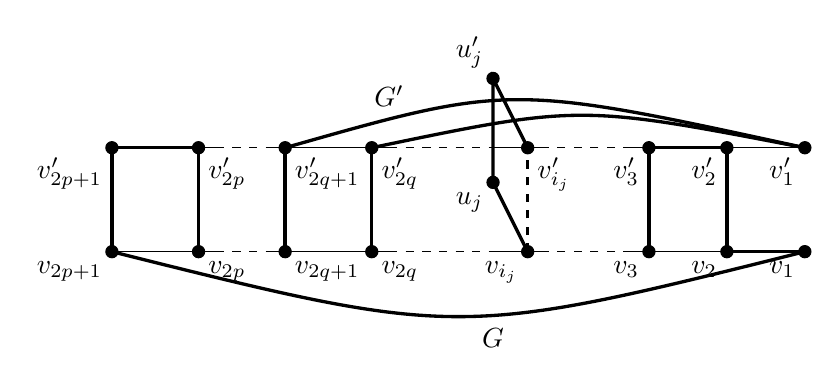
\begin{tikzpicture}[scale=2.2]
\draw(-2,0)node[below left]{$v_{2p+1}$}--(-1.4,0);\draw(1,0)--(2,0);
\draw(-2,0.6)node[below left]{$v'_{2p+1}$}--(-1.4,0.6);\draw(1,0.6)--(2,0.6);
\filldraw[black](0.4,0)node[below left]{$v_{i_j}$} circle(1pt);
\filldraw[black](0.4,0.6)node[below right]{$v'_{i_j}$} circle(1pt);
\filldraw[black](-2,0.6) circle(1pt);
\filldraw[black](2,0.6)node[below left]{$v'_1$} circle(1pt);
\filldraw[black](-1.5,0.6)node[below right]{$v'_{2p}$} circle(1pt);
\filldraw[black](1.55,0.6)node[below left]{$v'_2$} circle(1pt);
\filldraw[black](2,0)node[below left]{$v_1$} circle(1pt);
\filldraw[black](-2,0) circle(1pt);
\filldraw[black](1.55,0)node[below left]{$v_2$} circle(1pt);
\filldraw[black](-1.5,0)node[below right]{$v_{2p}$} circle(1pt);
\draw[dashed](-1.4,0)--(-1.1,0);\draw(-1.1,0)--(-0.4,0);\filldraw[black](-1,0)node[below right]{$v_{2q+1}$} circle(1pt);
\draw[dashed](1,0)--(0.5,0);
\draw[dashed](-1.4,0.6)--(-1.1,0.6);\draw(-1.1,0.6)--(-0.4,0.6);\filldraw[black](-1,0.6)node[below right]{$v'_{2q+1}$} circle(1pt);
\draw[dashed](1,0.6)--(0.5,0.6);
\filldraw[black](1.1,0)node[below left]{$v_3$} circle(1pt);
\filldraw[black](1.1,0.6)node[below left]{$v'_3$} circle(1pt);
\filldraw[black](0.2,0.4)node[below left]{$u_j$} circle(1pt);
\filldraw[black](0.2,1)node[above left]{$u'_j$} circle(1pt);
\draw[very thick](2,0)--(1.55,0)--(1.55,0.6)--(1.1,0.6)--(1.1,0);
\draw[very thick](0.4,0)--(0.2,0.4)--(0.2,1)--(0.4,0.6);
\draw[dashed, very thick](0.4,0)--(0.4,0.6);
\draw[very thick](-1.5,0)--(-1.5,0.6)--(-2,0.6)--(-2,0);
\draw[very thick](-2,0)..controls(0,-0.5)..(2,0);

\node at(0.2,-0.5){$G$};\node at (-0.4,0.9){$G'$};
\draw[dashed](-0.4,0)--(0.2,0);\draw(0.2,0)--(0.5,0);
\draw[dashed](-0.4,0.6)--(0.2,0.6);\draw(0.2,0.6)--(0.5,0.6);
\filldraw[black](-0.5,0)node[below right]{$v_{2q}$} circle(1pt);
\filldraw[black](-0.5,0.6)node[below right]{$v'_{2q}$} circle(1pt);
\draw[very thick](-0.5,0.6)..controls(0.7,0.85)..(2,0.6);
\draw[very thick](-1,0.6)..controls(0.3,0.97)..(2,0.6);
\draw[very thick](-0.5,0.6)--(-0.5,0);
\draw[very thick](-1,0.6)--(-1,0);

\end{tikzpicture}

\end{center}
\end{figure}


\end{proof}

The following lemma comes from \cite{broersma2014toughness}.
\begin{lemma}\cite[Theorem 4]{broersma2014toughness}\label{lembroet4}
A triangle-free, $2K_2$-free graph $G$ is Hamiltonian if and only if $G$ is 1-tough.
\end{lemma}

Now, suppose $G$ is a triangle-free $2K_2$-free graph, then Lemma \ref{lembroet4} has already proved that $G$ is Hamiltonian, so certainly is prism-Hamiltonian.

If $2K_2$-free graph $G$ is a tree, we can easily check that $G$ contains at most two vertices whose degree are at least two. So, if a $2K_2$-free tree is 1-tough, it can only be a single edge. There is nothing to prove.


If $2K_2$-free graph $G$ is not a tree and not triangle-free then by the second part of Theorem \ref{addgen1} and Lemma \ref{keylem}, we have finished the proof.
\qed











\section{On 2-walks in some other graphs}
As a generalization of $2K_2$-free graphs, let us look at $3K_2$-free graphs, which are the graphs without three vertex-disjoint edges as a induced subgraph.

In \cite{veldman83}, Veldman proved that:
\begin{lemma}\label{gen3k2de}{\cite[Corollary 3.2]{veldman83}}
Let $G$ be a 2-connected graph. If the degree sum of every three vertex-disjoint edges of $G$ is at least $|V(G)|-1$, then $G$ admits an edge-dominating cycle.
\end{lemma}

Combine Lemma \ref{gen3k2de} and Lemma \ref{addtec}, we get:

\begin{theorem}\label{2w3k2f}
Let $G$ be a 1-tough graph. If the degree sum of every three vertex-disjoint edges of $G$ is at least $|V(G)|-1$, then $G$ admits a 2-walk.
\end{theorem}

\begin{proof}
Clearly, if $G$ is 1-tough, then $G$ is 2-connected. So, by Lemma \ref{gen3k2de}, $G$ has an edge-dominating cycle. Thus, by Lemma \ref{addtec}, $G$ admits a 2-walk.
\end{proof}

Obviously, we get the following corollary.
\begin{corollary}
Every 1-tough $3K_2$-free graph admits a 2-walk.
\end{corollary}

Also in \cite{veldman83}, Veldman proved:

\begin{lemma}\label{lemdelta}{\cite[Theorem C]{veldman83}}
Let $G$ be a 2-connected graph, if the minimal degree $\delta\ge\frac{|V(G)|+2}{3}$, then every longest cycle of $G$ is edge-dominating.
\end{lemma}

\begin{lemma}\label{2conxiaoe}{\cite[Corollary 3.3.1]{veldman83}}
If $G$ is a 2-connected graph with $$|E(G)|\ge(\frac{(|V(G)|-4)(|V(G)|-5)}{2}+11),$$ then $G$ admits an edge-dominating cycle.
\end{lemma}

Obviously, combine Lemma \ref{addtec} with the two lemmas above, we get:

\begin{theorem}\label{mdeg2w}
For any 1-tough graph $G$, if the minimal degree $\delta\ge\frac{|V(G)|+2}{3}$, then $G$ admits a 2-walk.
\end{theorem}


\begin{theorem}
For any 1-tough graph $G$, if $$|E(G)|\ge(\frac{(|V(G)|-4)(|V(G)|-5)}{2}+11),$$ then $G$ admits a 2-walk.
\end{theorem}



What is more, our Lemma \ref{addtec} can also be applied on some other graphs, for example triangle-free graphs.

In \cite{aung1989longest} and \cite{ozeki2011dominating}, we find the following result.
\begin{lemma}\cite[Corollary 1.4]{aung1989longest}\label{lm89tr}
Any 2-connected triangle-free graph $G$ with $|G|\le6\delta-6$ contains a longest cycle which is also edge-dominating.
\end{lemma}

\begin{lemma}\cite[Theorem 6]{ozeki2011dominating}\label{lm11tr}
Any 2-connected triangle-free graph with $\alpha(G)\le2\kappa(G)-1$ contains a longest cycle which is also edge-dominating.
\end{lemma}

Obviously, combine Lemma \ref{addtec} with Lemma \ref{lm89tr} and Lemma \ref{lm11tr}, we ge the following result.
\begin{theorem}
Any 1-tough triangle-free graph $G$ with  $|G|\le6\delta-6$ admits a 2-walk.
\end{theorem}

\begin{theorem}
Any 1-tough triangle-free graph with  $\alpha(G)\le2\kappa(G)-1$ admits a 2-walk.
\end{theorem}



\subsection*{Acknowledgements.}
The authors thank Nick Gravin
for helpful comments on a draft of this text.
Research supported by Singapore MOE Tier 2 Grant MOE2011-T2-1-090 (ARC 19/11). 

\bibliography{reftough}
\bibliographystyle{abbrv}
%\bibliographystyle{plain}
\end{document}
